
% ----------------------------------------------------------------------
%                LATEX TEMPLATE FOR PhD THESIS AT STOCKHOLM UNIVERSITY
% ----------------------------------------------------------------------

% based on Harish Bhanderi's PhD/MPhil template, then Uni Cambridge
% http://www-h.eng.cam.ac.uk/help/tpl/textprocessing/ThesisStyle/
% corrected and extended in 2007 by Jakob Suckale, then MPI-CBG PhD programme
% and made available through OpenWetWare.org - the free biology wiki
% modified for SU by Andreas Solders in 2011

%: Style file for Latex
% Most style definitions are in the external filePhDthesisSU.
% In this template package, it can be found in ./Latex/Classes/

\documentclass[twoside,11pt]{Latex/Classes/PhDthesisSU} %Default style using S5 paper
%\documentclass[twoside,11pt]{Latex/Classes/PhDthesisSU_A4} %Use this instead if you need A4 paper.

%: Macro file for Latex
% Macros help you summarize frequently repeated Latex commands.
% Here, they are placed in an external file /Latex/Macros/MacroFile1.tex
% An macro that you may use frequently is the figuremacro
% This file contains macros that can be called up from connected TeX files
% It helps to summarise repeated code, e.g. figure insertion (see below).

% insert a centered figure with caption and description
% parameters 1:filename, 2:title, 3:description and label
\newcommand{\figuremacro}[3]{
	\begin{figure}[htbp]
		\centering
		\includegraphics[width=1\textwidth]{#1}
		\caption[#2]{\textbf{#2} - #3}
		\label{#1}
	\end{figure}
}

% insert a centered figure with caption and description AND WIDTH
% parameters 1:filename, 2:title, 3:description and label, 4: textwidth
% textwidth 1 means as text, 0.5 means half the width of the text
\newcommand{\figuremacroW}[4]{
	\begin{figure}[htbp]
		\centering
		\includegraphics[width=#4\textwidth]{#1}
		\caption[#2]{\textbf{#2} - #3}
		\label{#1}
	\end{figure}
}

% inserts a figure with wrapped around text; only suitable for NARROW figs
% o is for outside on a double paged document; others: l, r, i(inside)
% text and figure will each be half of the document width
% note: long captions often crash with adjacent content; take care
% in general: above 2 macro produce more reliable layout
\newcommand{\figuremacroN}[3]{
	\begin{wrapfigure}{o}{0.5\textwidth}
		\centering
		\includegraphics[width=0.48\textwidth]{#1}
		\caption[#2]{{\small\textbf{#2} - #3}}
		\label{#1}
	\end{wrapfigure}
}

% predefined commands by Harish
\newcommand{\PdfPsText}[2]{
  \ifpdf
     #1
  \else
     #2
  \fi
}

\newcommand{\IncludeGraphicsH}[3]{
  \PdfPsText{\includegraphics[height=#2]{#1}}{\includegraphics[bb = #3, height=#2]{#1}}
}

\newcommand{\IncludeGraphicsW}[3]{
  \PdfPsText{\includegraphics[width=#2]{#1}}{\includegraphics[bb = #3, width=#2]{#1}}
}

\newcommand{\InsertFig}[3]{
  \begin{figure}[!htbp]
    \begin{center}
      \leavevmode
      #1
      \caption{#2}
      \label{#3}
    \end{center}
  \end{figure}
}


%%% Local Variables: 
%%% mode: latex
%%% TeX-master: "~/Documents/LaTeX/CUEDThesisPSnPDF/thesis"
%%% End: 



\setcitestyle{square,numbers} % change how references are included (see the natbib package).

%: -------------------------------------------------------------
%:                  TITLE PAGE
% --------------------------------------------------------------

\title{Title of your thesis}%Title of the thesis
\subtitle{Subtitle}% Subtitle of the thesis
\author{\href{mailto:email@department.su.se}{Your Name}}

%put the following in PDF header

%\pdfinfo { /Title  ()
%               /Creator ()
%               /Producer ()
%               /Author ()
%               /CreationDate (D:YYYYMMDDhhmmss)  %format D:YYYYMMDDhhmmss
%               /ModDate (D:YYYYMMDDhhmm)
%               /Subject (xyz)
%               /Keywords (add, your, keywords, here) }
%\pdfcatalog { /PageMode (/UseOutlines)
%                  /OpenAction (fitbh)  }

\pdfinfo{
   /Author (Nicola Talbot)
   /Title  (Creating a PDF document using PDFLaTeX)
   /CreationDate (D:20040502195600)
   /Subject (PDFLaTeX)
   /Keywords (PDF;LaTeX)
}



% ---------------------------------------------------------------
       
% turn of those nasty overfull and underfull hboxes
\hbadness=10000
\hfuzz=50pt



% ---------------------------------------------------------------
%:                  FRONT MATTER: dedications, abstract,..
% ---------------------------------------------------------------

%\includeonly{X/filename} % Uncomment to only compile the specified files.

\begin{document}

\selectlanguage{english}

\frontmatterSU

\halftitlepage

%: ----------------------- Generate cover page ------------------------

\maketitle  % command to print the title page with above variables


%: ----------------------- Cover page back side ------------------------

\newpage
\thispagestyle{empty}


% Thesis Abstract -----------------------------------------------------

\begin{abstracts} %creates the abstract header

The abstract will be printed on the spikblad which will be folded into the printed thesis. However, if you feel it necessary to also have the abstract in the printed document put it here.

\end{abstracts}

% ---------------------------------------------------------------------- 
 % Uncomment to input the abstract if you want to have it printed.

\phantom{.}

\vspace{\stretch{1}}

{\fontfamily{verdana}\selectfont
{\scriptsize
\noindent
\copyright Your Name, Stockholm 20XX % Name of author, location year
 
\vspace{5mm}
\noindent
ISBN XXX-XX-XXXX-XXX-X % Provided by the library

\vspace{5mm}
\noindent
Printed in Sweden by XXXX, Stockholm 2011 %name of printing company

\noindent
Distributor: Department of XX, Stockholm University %name of department
}
}
\cleardoublepage


%: ----------------------- Tie in front matter ------------------------

% Thesis Dedictation ---------------------------------------------------

\begin{dedication}

{\fontfamily{calligra}\selectfont
{\Large

This thesis is dedicated to...

}
}
\end{dedication}

% ---------------------------------------------------------------------- % Include a page with dedication

\chapter{List of Papers}

\vspace{-5pt} % Increase to have a larger space. 

The following papers, referred to in the text by their Roman numerals, are included in this thesis.

\vspace{0pt} % Increase to have a larger space before the list is started. 


\begin{enumerate}[P{A}PER I: ]
%\begin{enumerate}[I]

\setlength{\itemsep}{3.3mm} %Set the vertical distance between the items

        % Suggested order
        % Author 1 surname, Author 2 first name initial., Author 1 surname, Author 2 first name
        % initial. etc. (Year of publication) Paper main title.
        % Paper subtitle. Name of journal in italics, volume(number):page rage
        % Example


\item\textbf{Titel}\\
Author1, Author2, \emph{paper}, \textbf{issue}, page (YEAR).\\
DOI: \href{}{} 

\end{enumerate}

\noindent
\rule{\linewidth}{0.5mm}

\vspace{2mm}

\noindent
Reprints were made with permission from the publishers.



 % Include a list of papers


% Author's contribution -----------------------------------------------------

\chapter{Author's contribution}

If you want to include a summary of your contributions to the presented work in the frontmatter, put it here.


% ---------------------------------------------------------------------- 
 % Include a page with authors contribution


%: ----------------------- Table of contents ------------------------

\setcounter{secnumdepth}{2} % organisational level that receives a numbers
\setcounter{tocdepth}{2}    % print table of contents for level 2
\tableofcontents            % print the table of contents
% levels are: 0 - chapter, 1 - section, 2 - subsection, 3 - subsubsection



%: ----------------------- Abbreviations ------------------------

% Tie in external source file for definitions: /0_frontmatter/abbreviations.tex
% Abbreviation entries can also be defined in the main text. See abbreviations.tex
% To create the glossary run "makeindex thesis.nlo  -s nomencl.ist -o thesis.nls"

\renewcommand{\nomname}{Abbreviations} % Change title of page from Nomenclature to Abbreviations

%\nomrefpage % to include page numbers after abbrevations

% In the text type "\g" to refer to glossary

% this file is called up by thesis.tex
% content in this file will be fed into the main document

% Glossary entries are defined with the command \nomenclature{1}{2}
% 1 = Entry name, e.g. abbreviation; 2 = Explanation
% You can place all explanations in this separate file or declare them in the middle of the text. Either way they will be collected in the glossary.

% required to print nomenclature name to page header
\markboth{\MakeUppercase{\nomname}}{\MakeUppercase{\nomname}}


% ----------------------- contents from here ------------------------

%

\nomenclature{LaTeX}{Lamport TeX}







%\begin{multicols}{2}  % uncomment to have 2 columns

\begin{footnotesize} % scriptsize(7) < footnotesize(8) < small (9) < normal (10)

\printnomenclature[2 cm] % [] = distance between entry and description
\label{nom} % target name for links to glossary

\end{footnotesize}

%\end{multicols}

%: ----------------------- list of figures/tables ------------------------

\listoffigures	% print list of figures

\listoftables  % print list of tables

%: ----------------------- Acknowledgements ------------------------

% Thesis Acknowledgements ------------------------------------------------


\chapter{Acknowledgements}

I would like to acknowledge...



% ------------------------------------------------------------------------


 % Use this to include an acknowledgement in the frontmatter



%: --------------------------------------------------------------
%:                  MAIN DOCUMENT SECTION
% --------------------------------------------------------------

% the main text starts here with the introduction, 1st chapter,...

\mainmatterSU


%: ----------------------- subdocuments ------------------------

% Parts of the thesis are included below. Rename the files as required.
% But take care that the paths match. You can also change the order of appearance by moving the include commands.

% this file is called up by thesis.tex
% content in this file will be fed into the main document

%: ----------------------- introduction file header -----------------------

\graphicspath{{1_introduction/figures/}} % specifies where the figures are stored

% ----------------------------------------------------------------------
%: ----------------------- content ----------------------- 
% ----------------------------------------------------------------------



%: ----------------------- HELP: latex document organisation
% the commands below help you to subdivide and organise your thesis
%    \chapter{}       = level 1, top level
%    \section{}       = level 2
%    \subsection{}    = level 3
%    \subsubsection{} = level 4
% note that everything after the percentage sign is hidden from output



\chapter{Introduction} % top level followed by section, subsection


\section{What is this?}  

This is a template for producing PhD-thesis at Stockholm University (SU)\nomenclature{SU}{Stockholm University} using pdf\LaTeX. It could also, with some alterations, be used for Master thesis and Licentiat thesis. Observe that it is designed to be used with pdf\LaTeX and will not work (at least not as in the present state) with \TeX,\LaTeX or pdf\TeX.

The template produces all necessary parts such as half title page, title page, printing info and so on. Simply input the information as called for in the file \emph{thesis.tex}. It also produces a number of parts for the front matter and back matter. Some of these parts are mandatory and some are optional depending on whether it is a monograph or a summary dissertation. Comment or uncomment these to fit your preferences. 



%\subsection{Name your subsection} % subsection headings are again smaller than section names
%\subsubsection{Name your subsubsection} % subsubsection headings are again smaller than subsection names








%Starch of plants and glycogen of animals consists of $\alpha$-1,4-glycosidic glucose polymers \cite{lastname07}. See figure \ref{largepotato} for a comparison of glucose polymer structure and chemistry. 

%Two references can be placed separated by a comma \cite{lastname07,name06}.

%: ----------------------- HELP: references
% References can be links to figures, tables, sections, or references.
% For figures, tables, and text you define the target of the link with \label{XYZ}. Then you call cross-link with the command \ref{XYZ}, as above
% Citations are bound in a very similar way with \cite{XYZ}. You store your references in a BibTex file with a programme like BibDesk.





%\figuremacro{largepotato}{A common glucose polymers}{The figure shows starch granules in potato cells, taken from \href{http://molecularexpressions.com/micro/gallery/burgersnfries/burgersnfries4.html}{Molecular Expressions}.}

%: ----------------------- HELP: adding figures with macros
% This template provides a very convenient way to add figures with minimal code.
% \figuremacro{1}{2}{3}{4} calls up a series of commands formating your image.
% 1 = name of the file without extension; PNG, JPEG is ok; GIF doesn't work
% 2 = title of the figure AND the name of the label for cross-linking
% 3 = caption text for the figure

%: ----------------------- HELP: www links
% You can also see above how, www links are placed
% \href{http://www.something.net}{link text}

	%\figuremacroW{largepotato}{Title}{Caption}{0.8}

% variation of the above macro with a width setting
% \figuremacroW{1}{2}{3}{4}
% 1-3 as above
% 4 = size relative to text width which is 1; use this to reduce figures




%: ----------------------- HELP: tables
% Directly coding tables in latex is tiresome. See below.
% I would recommend using a converter macro that allows you to make the table in Excel and convert them into latex code which you can then paste into your doc.
% This is the link: http://www.softpedia.com/get/Office-tools/Other-Office-Tools/Excel2Latex.shtml
% It's a Excel template file containing a macro for the conversion.

%\begin{table}[htdp]
%\centering
%\begin{tabular}{ccc} % ccc means 3 columns, all centered; alternatives are l, r

%{\bf Gene} & {\bf GeneID} & {\bf Length} \\ 
% & denotes the end of a cell/column, \\ changes to next table row
%\hline % draws a line under the column headers

%human latexin & 1234 & 14.9 kbps \\
%mouse latexin & 2345 & 10.1 kbps \\
%rat latexin   & 3456 & 9.6 kbps \\
% Watch out. Every line must have 3 columns = 2x &. 
% Otherwise you will get an error.

%\end{tabular}
%\caption[title of table]{\textbf{title of table} - Overview of latexin genes.}
% You only need to write the title twice if you don't want it to appear in bold in the list of tables.
%\label{latexin_genes} % label for cross-links with \ref{latexin_genes}
%\end{table}



% There you go. You already know the most important things.


% ----------------------------------------------------------------------




\include{2/chapter2}
%% this file is called up by thesis.tex
% content in this file will be fed into the main document

%: ----------------------- introduction file header -----------------------

\graphicspath{{1_introduction/figures/}} % specifies where the figures are stored

% ----------------------------------------------------------------------
%: ----------------------- content ----------------------- 
% ----------------------------------------------------------------------

\chapter{Instructions} % top level followed by section, subsection

\section{Outline of the thesis \label{layout}}

The outline of the thesis depends on whether it is a monograph or a summary. The different parts of the two types of thesis are summarized in Table\ref{tab:outline} were the optional parts have been put in italics. In this template all parts have been included and it is up to the author to exclude (comment) the appropriate parts in the main file \emph{thesis.tex}. The different parts of the thesis are described in the following sections.

% to tell LaTeX we want to use our table as a float, we need to put a table environment around the tabular environment
% https://en.wikibooks.org/wiki/LaTeX/Tables
\begin{table}[htbp]
\begin{tabular}{|l|l|}
\hline
\textbf{Summary} & \textbf{Monograph} \\
Title page & Half title page \\
Printing info (\emph{abstract}) & Empty page \\
\emph{Dedication page} & Title page \\
Possible empty page & Printing info (\emph{abstract}) \\
List of papers & \emph{Dedication page} \\
Possible empty page & Possible empty page \\
\emph{Authors contribution} & Table of contents \\
Possible empty page & Possible empty page \\
Table of contents & \emph{List of Abbreviations/Figures/Tables} \\
Possible empty page & Possible empty page \\
\emph{List of Abbreviations/Figures/Tables}  & \emph{Acknowledgments} \\
Possible empty page & Possible empty page \\
Chapter 1 introduction & Chapter 1 introduction\\
Chapter 2...N & Chapter 2...N\\
Summary & Summary \\
\emph{Acknowledgments} & References \\
References & \\
\hline

\end{tabular}
\caption{\label{tab:outline}Outline of the two types of thesis. Parts in italics are optional.}
\end{table}

\subsection{Title page}
This should include the SU logotype, thesis title and subtitle as well as the name of the author. The page is automatically generated by the template using information supplied by the author in the file \emph{thesis.tex}.

\subsection{Half title page}
This page (smutstittelsida) is generated by the command 
\begin{verbatim}
\halftitlepage
\end{verbatim}
in \emph{thesis.tex}.

\subsection{Printing info (abstract)}
The printing info should be supplied by the author in the file \emph{thesis.tex}. The abstract of the thesis will be printed on the spikblad which will be generated upon the electronic spikning. However, if the author believes it necessary to also include the abstract in the printed document this is were it should go. The body of the abstract should the be included in the file \emph{abstract.tex} in \emph{$\backslash$0\_frontmatter}.

\subsection{Dedication}
If you would like to include a dedication put the text in the file \emph{dedication.tex} in \emph{$\backslash$0\_frontmatter}. If not, comment the line 
\begin{verbatim}
\include 0_frontmatter/dedication
\end{verbatim}
in \emph{thesis.tex}.

\subsection{List of papers}
Same as Dedication.

\subsection{Authors contribution}
Same as Dedication

\subsection{Table of contents}
Automatically generated by \emph{thesis.tex}.

\subsection{List of Abbreviations/Figures/Tables}
These lists can be included or excluded according to the authors wishes. List of figures and List of Tables are automatically generated by corresponding commands in \emph{thesis.tex}. The List of Abbreviations is also generated by \emph{thesis.tex} using the file \emph{thesis.nls}. This can in turn be generated by the command 'makeindex thesis.nlo  -s nomencl.ist -o thesis.nls' from the file \emph{thesis.nlo} which is automatically generated by pdf\LaTeX from the entries found in the file \emph{abbreviations.tex} in  \emph{$\backslash$0\_frontmatter} or in any of the included .tex-files using the syntax
\begin{verbatim}
\nomenclature{STHML}{Stockholm}.
\end{verbatim}
\nomenclature{STHML}{Stockholm} For more information see the documatation of the \emph{nomencl} package \citep{nomencl}

\subsection{Acknowledgements}
If you are writing a Monograph and would like to add acknowledgements this is were you put it. Simply make sure the line
\begin{verbatim}
% Thesis Acknowledgements ------------------------------------------------


\chapter{Acknowledgements}

I would like to acknowledge...



% ------------------------------------------------------------------------


 
\end{verbatim}
in the Front matter part of \emph{thesis.tex} and edit the file  \emph{acknowledgement.tex} in \emph{$\backslash$0\_frontmatter}.

\subsection{Chapter 1...N}
The chapters are included in the Main matter part of \emph{thesis.tex}. To help you organize your document it is recommended that each chapter is put in separate file in a folder of its own.

\subsection{Summary}
A short summary in Swedish should be be included if the thesis is written in a foreign language.

\subsection{Acknowledgements}
If you are writing a Summary and would like to add acknowledgements this is were you put it. Simply make sure the line
\begin{verbatim}
% Thesis Acknowledgements ------------------------------------------------


\chapter{Acknowledgements}

I would like to acknowledge...



% ------------------------------------------------------------------------


 
\end{verbatim}
in the Back matter part of \emph{thesis.tex} is not commented and edit the file  \emph{acknowledgement.tex} in \emph{$\backslash$0\_frontmatter}.

\subsection{References}
Put you references in the Bib\TeX-file \emph{references.bib} in \emph{9\_backmatter}. A few Bib\TeX style files are included in \emph{$\backslash$Latex$\backslash$Classes} but the author a free to use the bibliographic style of her/his preference. More information on how to use Bib\TeX can be found at the Bib\TeX  homepage \citep{bibtex}.

% ---------------------------------------------------------------------------
%: ----------------------- end of thesis sub-document ------------------------
% ---------------------------------------------------------------------------

				
%% this file is called up by thesis.tex
% content in this file will be fed into the main document

%: ----------------------- introduction file header -----------------------

\graphicspath{{3/figures/}} % specifies where the figures are stored

% ----------------------------------------------------------------------
%: ----------------------- content ----------------------- 
% ----------------------------------------------------------------------

\chapter{\label{ch3}Name of chapter 3} % top level followed by section, subsection

Lorem ipsum dolor sit amet, consectetur adipisicing elit, sed do eiusmod tempor incididunt ut labore et dolore magna aliqua. Ut enim ad minim veniam, quis nostrud exercitation ullamco laboris nisi ut aliquip ex ea commodo consequat. Duis aute irure dolor in reprehenderit in voluptate velit esse cillum dolore eu fugiat nulla pariatur. Excepteur sint occaecat cupidatat non proident, sunt in culpa qui officia deserunt mollit anim id est laborum.

\section{\label{}Name of section}

Lorem ipsum dolor sit amet, consectetur adipisicing elit, sed do eiusmod tempor incididunt ut labore et dolore magna aliqua. Ut enim ad minim veniam, quis nostrud exercitation ullamco laboris nisi ut aliquip ex ea commodo consequat. Duis aute irure dolor in reprehenderit in voluptate velit esse cillum dolore eu fugiat nulla pariatur. Excepteur sint occaecat cupidatat non proident, sunt in culpa qui officia deserunt mollit anim id est laborum \ref{fig:potato}.

\begin{figure}[htbp]
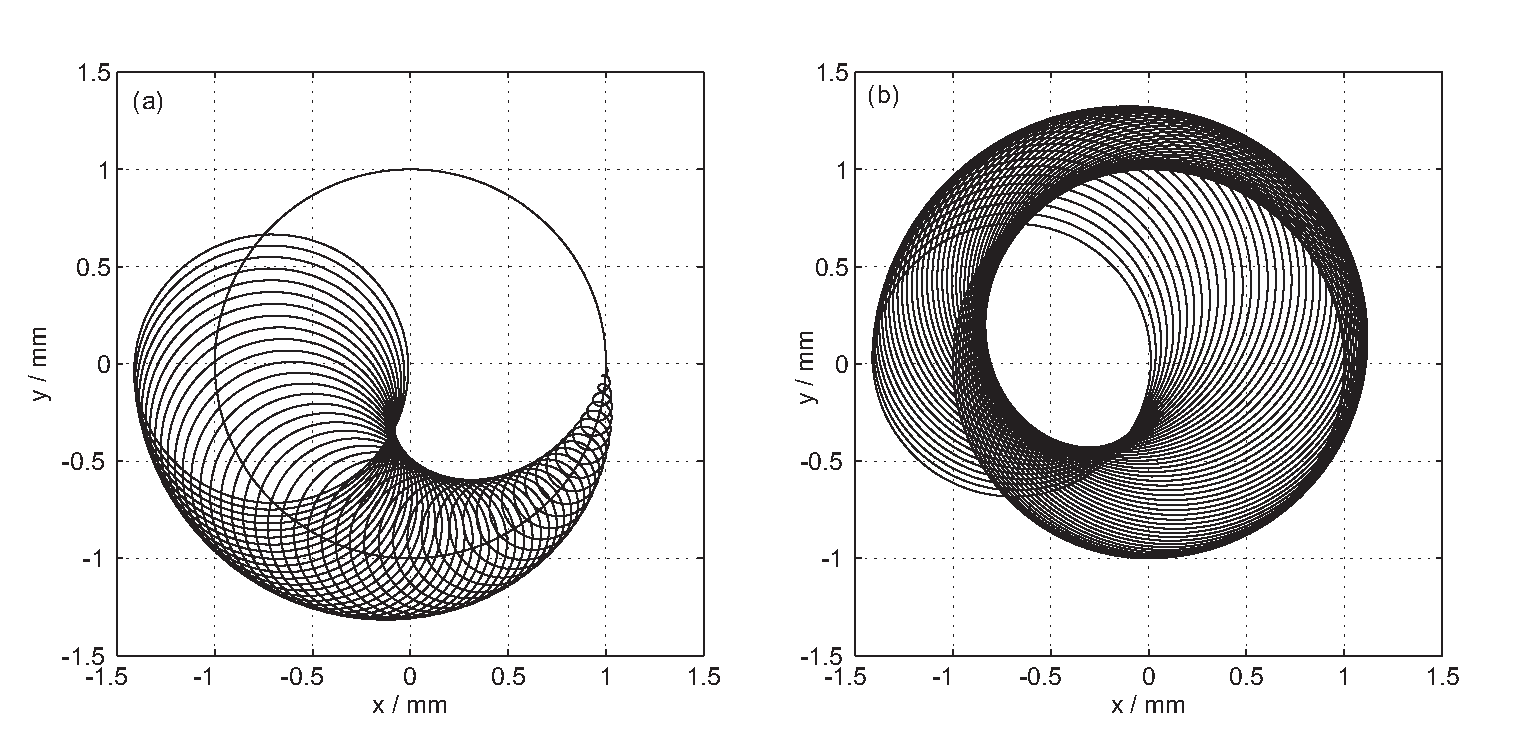
\includegraphics[width=\textwidth]{conversion.eps}
\caption{\label{fig:potato}Example figure}
\end{figure}

Lorem ipsum dolor sit amet, consectetur adipisicing elit, sed do eiusmod tempor incididunt ut labore et dolore magna aliqua. Ut enim ad minim veniam, quis nostrud exercitation ullamco laboris nisi ut aliquip ex ea commodo consequat. Duis aute irure dolor in reprehenderit in voluptate velit esse cillum dolore eu fugiat nulla pariatur. Excepteur sint occaecat cupidatat non proident, sunt in culpa qui officia deserunt mollit anim id est laborum.

\subsection{\label{}Name of subsection}

Lorem ipsum dolor sit amet, consectetur adipisicing elit, sed do eiusmod tempor incididunt ut labore et dolore magna aliqua. Ut enim ad minim veniam, quis nostrud exercitation ullamco laboris nisi ut aliquip ex ea commodo consequat. Duis aute irure dolor in reprehenderit in voluptate velit esse cillum dolore eu fugiat nulla pariatur. Excepteur sint occaecat cupidatat non proident, sunt in culpa qui officia deserunt mollit anim id est laborum.

Lorem ipsum dolor sit amet, consectetur adipisicing elit, sed do eiusmod tempor incididunt ut labore et dolore magna aliqua. Ut enim ad minim veniam, quis nostrud exercitation ullamco laboris nisi ut aliquip ex ea commodo consequat. Duis aute irure dolor in reprehenderit in voluptate velit esse cillum dolore eu fugiat nulla pariatur. Excepteur sint occaecat cupidatat non proident, sunt in culpa qui officia deserunt mollit anim id est laborum.

\subsubsection{\label{}Name of subsubsection}

Lorem ipsum dolor sit amet, consectetur adipisicing elit, sed do eiusmod tempor incididunt ut labore et dolore magna aliqua. Ut enim ad minim veniam, quis nostrud exercitation ullamco laboris nisi ut aliquip ex ea commodo consequat. Duis aute irure dolor in reprehenderit in voluptate velit esse cillum dolore eu fugiat nulla pariatur. Excepteur sint occaecat cupidatat non proident, sunt in culpa qui officia deserunt mollit anim id est laborum.


% ---------------------------------------------------------------------------
%: ----------------------- end of thesis sub-document ------------------------
% ---------------------------------------------------------------------------

	
%% this file is called up by thesis.tex
% content in this file will be fed into the main document

%: ----------------------- introduction file header -----------------------

\graphicspath{{4/figures/}} % specifies where the figures are stored

% ----------------------------------------------------------------------
%: ----------------------- content ----------------------- 
% ----------------------------------------------------------------------

\chapter{\label{ch4}Name of chapter 4} % top level followed by section, subsection

\section{\label{}Name of section}

\subsection{\label{}Name of subsection}



% ---------------------------------------------------------------------------
%: ----------------------- end of thesis sub-document ------------------------
% ---------------------------------------------------------------------------

	
%% this file is called up by thesis.tex
% content in this file will be fed into the main document

%: ----------------------- introduction file header -----------------------

\graphicspath{{5/figures/}} % specifies where the figures are stored

% ----------------------------------------------------------------------
%: ----------------------- content ----------------------- 
% ----------------------------------------------------------------------

\chapter{\label{ch5}Name of chapter 5} % top level followed by section, subsection

\section{\label{}Name of section}

\subsection{\label{}Name of subsection}



% ---------------------------------------------------------------------------
%: ----------------------- end of thesis sub-document ------------------------
% ---------------------------------------------------------------------------

	
%% this file is called up by thesis.tex
% content in this file will be fed into the main document

%: ----------------------- introduction file header -----------------------

\graphicspath{{6/figures/}} % specifies where the figures are stored

% ----------------------------------------------------------------------
%: ----------------------- content ----------------------- 
% ----------------------------------------------------------------------

\chapter{\label{ch6}Name of chapter 6} % top level followed by section, subsection

\section{\label{}Name of section}

\subsection{\label{}Name of subsection}



% ---------------------------------------------------------------------------
%: ----------------------- end of thesis sub-document ------------------------
% ---------------------------------------------------------------------------

	
%% this file is called up by thesis.tex
% content in this file will be fed into the main document

%: ----------------------- introduction file header -----------------------

\graphicspath{{7/figures/}} % specifies where the figures are stored

% ----------------------------------------------------------------------
%: ----------------------- content ----------------------- 
% ----------------------------------------------------------------------

\chapter{\label{ch7}Name of chapter 7} % top level followed by section, subsection

\section{\label{}Name of section}

\subsection{\label{}Name of subsection}



% ---------------------------------------------------------------------------
%: ----------------------- end of thesis sub-document ------------------------
% ---------------------------------------------------------------------------

	
            
% Include as many chapters as you need
     




% --------------------------------------------------------------
%:                  BACK MATTER: appendices, refs,..
% --------------------------------------------------------------

\backmatterSU

% the back matter: summary and references close the thesis


% Thesis summary -------------------------------------

% Should be in swedish if thesis are in another language, otherwize in english.
\selectlanguage{swedish}

%\summarytitle{Summering}

%\begin{summary}        %this creates the heading for the declaration page
\chapter{Sammanfattning}

En kort summering av avhandlingen p\r{a} svenska om avhandlingen \"ar skriven p\r{a}  ett annat spr\r{a}k.

\r{a} \"a \"o




%\end{summary}

\selectlanguage{english}

% ----------------------------------------------------------------------

% Thesis Acknowledgements ------------------------------------------------


%\begin{acknowledgementslong} %uncommenting this line, gives a different acknowledgements heading
%\begin{acknowledgements}      %this creates the heading for the acknowlegments
\chapter{Acknowledgements}

I would like to acknowledge...

%\end{acknowledgements}
%\end{acknowledgmentslong}

% ------------------------------------------------------------------------


  % Use this to include an acknowledgement in the backmatter

%: ----------------------- bibliography ------------------------

% The section below defines how references are listed and formatted.


%\begin{multicols}{2} % \begin{multicols}{ # columns}[ header text][ space] %uncomment to have 2 columns
\begin{scriptsize} % tiny(5) < scriptsize(7) < footnotesize(8) < small (9)

\bibliographystyle{Latex/Classes/PhDbiblio-url2} %Default style file. Change according to you preferences.


\renewcommand{\bibname}{References} % changes the header from Bibliography to References

\bibliography{9_backmatter/references} % adjust this to fit your BibTex file

\end{scriptsize}
%\end{multicols}


% Various bibliography styles exit. Replace above style as desired.

% in-text refs: (1) (1; 2)
% ref list: alphabetical; author(s) in small caps; initials last name; page(s)
%\bibliographystyle{Latex/Classes/PhDbiblio-case} % title forced lower case
%\bibliographystyle{Latex/Classes/PhDbiblio-bold} % title as in bibtex but bold
%\bibliographystyle{Latex/Classes/PhDbiblio-url} % bold + www link if provided
%\bibliographystyle{Latex/Classes/jmb} % calls style file jmb.bst
% in-text refs: author (year) without brackets
% ref list: alphabetical; author(s) in normal font; last name, initials; page(s)

%\bibliographystyle{plainnat} % calls style file plainnat.bst
% in-text refs: author (year) without brackets
% (this works with package natbib)


% --------------------------------------------------------------



\end{document}
